% !TEX program = xelatex
% 丙午稗史 / Bingwu Baishi - Classic literary edition
% Compile: latexmk -xelatex -interaction=nonstopmode -halt-on-error main.tex
\documentclass[UTF8,11pt,twoside,openright,fontset=none]{ctexbook}
\usepackage[a5paper,inner=22mm,outer=19mm,top=22mm,bottom=22mm,headheight=16pt,headsep=7mm,footskip=12mm]{geometry}
\usepackage{fontspec}
\setmainfont{TeXGyrePagella}
\setCJKmainfont[AutoFakeBold=2]{Noto Serif CJK SC}
\setCJKsansfont{Noto Sans CJK SC}
\setCJKmonofont{Noto Sans Mono CJK SC}
\newCJKfontfamily\headfont[AutoFakeBold=2]{Noto Serif CJK SC}
\newCJKfontfamily\titlefont[AutoFakeBold=3]{Noto Serif CJK SC}
\newfontfamily\symbolsfont{DejaVu Sans}
\newfontfamily\javanesefont{Noto Sans Javanese}
\usepackage{tikz}
\usetikzlibrary{calc,decorations.pathmorphing}
\usepackage{xcolor}
\definecolor{navy}{HTML}{101C27}
\definecolor{bookgold}{HTML}{E4C88B}
\definecolor{oldgold}{HTML}{A68550}
\definecolor{wine}{HTML}{823F38}
\definecolor{ink}{HTML}{252A29}
\definecolor{muted}{HTML}{736D62}
\definecolor{quoteedge}{HTML}{B6A48B}
\definecolor{quoteivory}{HTML}{FAF8F3}
\usepackage{graphicx}
\usepackage{microtype}
\usepackage{needspace}
\usepackage{mdframed}
\usepackage{fancyhdr}
\usepackage{titlesec}
\usepackage{tocloft}
\usepackage{hyperref}
\usepackage{bookmark}
\hypersetup{unicode=true,pdfauthor={海生不浪},pdftitle={丙午稗史},pdfsubject={网络伪史异说汇编与辨析},colorlinks=true,linkcolor=wine,urlcolor=wine,bookmarksopen=true,bookmarksnumbered=false}
\setcounter{tocdepth}{0}
\setlength{\parindent}{2em}
\setlength{\parskip}{0pt}
\linespread{1.45}
\setlength{\emergencystretch}{3em}
\sloppy
\renewcommand{\contentsname}{卷目}
\renewcommand{\cftchapfont}{\normalfont\headfont}
\renewcommand{\cftchappagefont}{\normalfont}
\renewcommand{\cftchapleader}{\cftdotfill{1.5}}
\setlength{\cftbeforechapskip}{10pt}
\fancyhf{}
\fancyhead[LE]{\footnotesize\headfont\color{muted}丙午稗史}
\fancyhead[RO]{\footnotesize\headfont\color{muted}\leftmark}
\fancyfoot[LE,RO]{\color{wine}\thepage}
\renewcommand{\headrulewidth}{.35pt}
\renewcommand{\footrulewidth}{0pt}
\pagestyle{fancy}
\fancypagestyle{plain}{\fancyhf{}\fancyfoot[C]{\color{wine}\thepage}\renewcommand{\headrulewidth}{0pt}}
\newcommand{\ornament}{\tikz[baseline=-0.6ex]{\draw[oldgold,line width=.5pt](-1.7,0)--(-.3,0);\fill[oldgold] (0,0) --(.13,.13)--(.26,0)--(.13,-.13)--cycle;\draw[oldgold,line width=.5pt](.42,0)--(1.82,0);}}
% front/back sections
\newcommand{\BookPart}[1]{%
 \cleardoublepage\phantomsection\addcontentsline{toc}{chapter}{#1}\markboth{#1}{#1}%
 \thispagestyle{plain}%
 \begin{center}\vspace*{10mm}{\fontsize{26}{38}\titlefont\color{ink}#1}\par\vspace{5mm}\ornament\end{center}\vspace{10mm}%
}
% Each volume begins on an individually typeset recto opener.
\newcommand{\BookVolume}[3]{%
 \cleardoublepage\phantomsection\addcontentsline{toc}{chapter}{卷之#1·#2}\markboth{卷之#1·#2}{卷之#1·#2}%
 \thispagestyle{empty}\null\vspace*{25mm}%
 \begin{center}
 {\color{oldgold}\headfont\Large 卷之#1}\par
 \vspace{18mm}
 {\titlefont\fontsize{82}{90}\selectfont\color{ink}#2}\par
 \vspace{13mm}\ornament\par
 \vspace{12mm}{\color{muted}\small #3}\par
 \end{center}
 \vfill
 \begin{center}{\scriptsize\color{muted}丙午岁\quad 九卷汇编}\end{center}
 \clearpage
}
% Paragraph-long primary quotations are breakable across pages
\newenvironment{sourcequote}{%
\begin{mdframed}[linecolor=quoteedge,linewidth=.7pt,topline=false,rightline=false,bottomline=false,backgroundcolor=quoteivory,skipabove=5pt,skipbelow=11pt,innerleftmargin=10pt,innerrightmargin=7pt,innertopmargin=7pt,innerbottommargin=7pt,splittopskip=8pt,splitbottomskip=8pt]%
\begingroup\fontsize{10.5pt}{17pt}\selectfont\color{ink}\parindent=1.6em
}{\par\endgroup\end{mdframed}}
\newcommand{\SourceEntry}[3]{%
\par\Needspace{5\baselineskip}\vspace{8pt}%
\noindent\textcolor{wine}{\headfont\large #1}\hspace{1.1em}{\headfont\small #2}\par\nobreak\vspace{2pt}%
\begin{sourcequote}#3\end{sourcequote}
}
\newenvironment{verseblock}{\begin{center}\fontsize{12}{23}\selectfont\headfont\color{wine}}{\end{center}}
\begin{document}
\pagenumbering{gobble}
% Jacket-style front cover: image is original project artwork; title is selectable text.
\begin{titlepage}
\thispagestyle{empty}
\begin{tikzpicture}[remember picture,overlay]
 \node[anchor=center,inner sep=0pt] at (current page.center){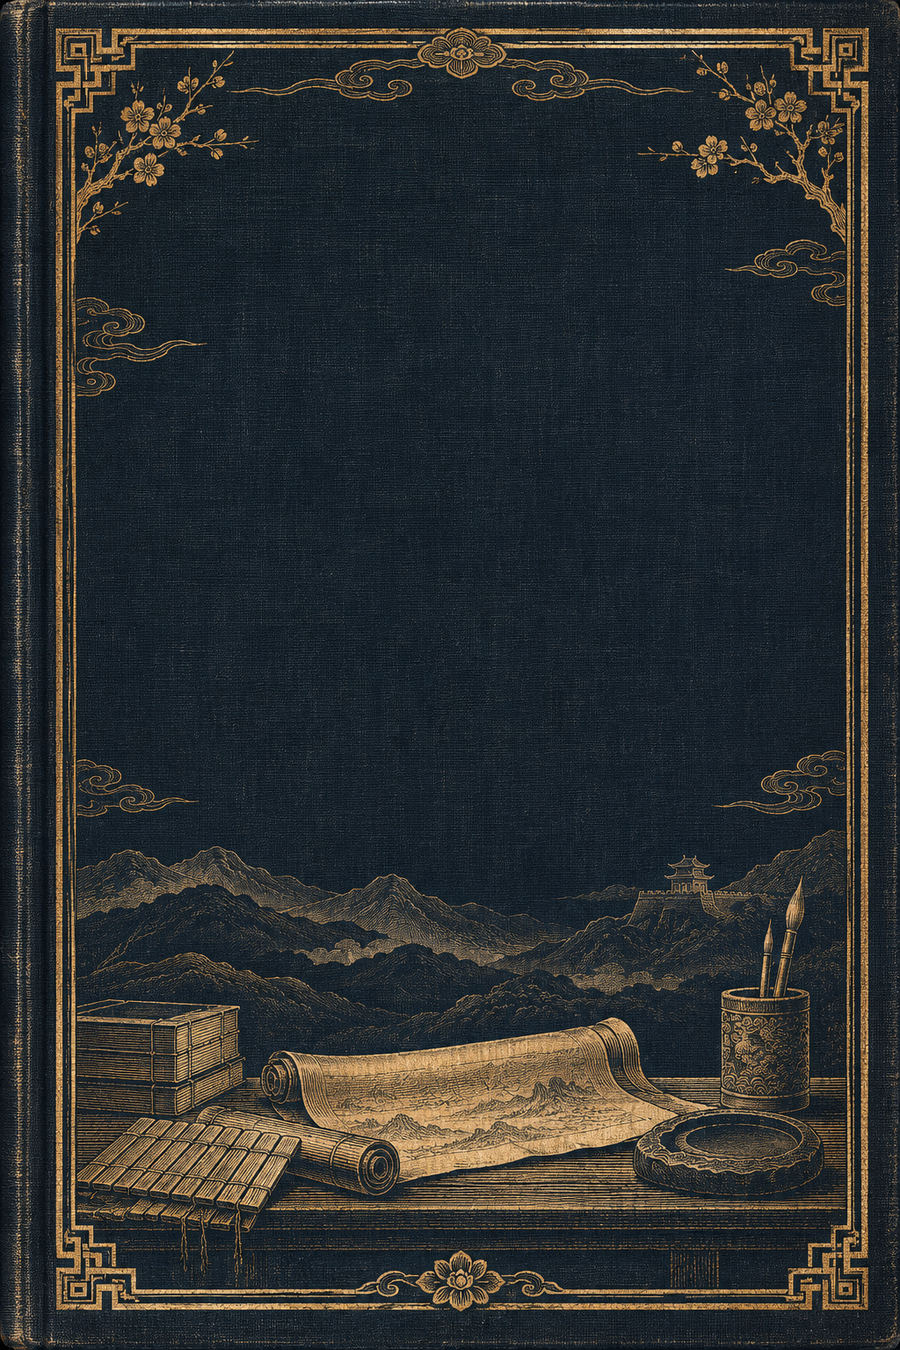
\includegraphics[width=\paperwidth,height=\paperheight]{assets/cover-art.jpg}};
 \node[anchor=north,text=bookgold] at ([yshift=-64mm]current page.north){\titlefont\fontsize{39}{52}\selectfont 丙午稗史};
 \node[anchor=north,text=bookgold] at ([yshift=-94mm]current page.north){\headfont\fontsize{11}{18}\selectfont 网 络 异 闻 · 丙 午 初 编};
 \node[anchor=north,text=bookgold] at ([yshift=-120mm]current page.north){\headfont\fontsize{12}{18}\selectfont 海生不浪\quad 编};
\end{tikzpicture}
\end{titlepage}
\newpage
\thispagestyle{empty}
\vspace*{15mm}
\begin{center}
{\fontsize{25}{34}\selectfont\CJKfontspec{Noto Serif CJK SC}丙午稗史}\par
\vspace{10mm}
{\color{oldgold}\rule{52mm}{0.7pt}}\par
\vspace{7mm}
{\Large 世有奇谈，姑录其言；\\[5pt]真伪未定，留待后贤。}\par
\end{center}
\vfill
\begin{center}
{\large 海生不浪\quad 编}\par
\vspace{4mm}
{\small 丙午岁\quad 二〇二六年}\par
\end{center}
\vspace*{14mm}
\clearpage
\thispagestyle{empty}
\vspace*{38mm}
{\small\color{muted}
\noindent\textbf{书名}\quad 丙午稗史\\[6pt]
\noindent\textbf{编纂}\quad 海生不浪\\[6pt]
\noindent\textbf{底本}\quad GitHub 项目 Bingwu-Baishi（初编）\\[6pt]
\noindent\textbf{版本}\quad 二〇二六年十一月，数字排印本\\[6pt]
\noindent\textbf{项目}\quad \href{https://github.com/ZJY-HSBL/Bingwu-Baishi}{github.com/ZJY-HSBL/Bingwu-Baishi}\\[10pt]
\noindent 本书为非正式出版的网络文献编纂稿；无 ISBN，不代表经出版社审校或学术同行评议。网络引文的原作者及权利归属，以可核实的原始来源为准。
\par\vspace{9mm}
\noindent 所录涉及种族歧视、非人化与暴力鼓动的材料，仅作为待核验的网络语料保存并加以批判，不代表编者认同。署名来自样本，未逐一核验，亦不应据之作现实身份指认。
}
\vfill
\noindent{\color{oldgold}\rule{\textwidth}{0.5pt}}
{\footnotesize\color{muted}排印建议：XeLaTeX · A5 双面阅读版 · 内文采用宋体。}
\clearpage
\thispagestyle{empty}
\vspace*{57mm}
\begin{center}
\color{wine}\fontsize{19}{33}\selectfont
史或可伪，言终有迹；\\
山河依旧，人心可书。
\end{center}
\vspace*{48mm}
\clearpage

\frontmatter
\pdfbookmark[0]{卷目}{book-toc}
\tableofcontents
\cleardoublepage
\BookPart{序}
岁在丙午，时维二〇二六年。

是岁也，九州风起，四海云兴。中国之人，似于一夕之间，忽寻得失落千载之根，洞悉湮没万世之史。昔之所学，尽成疑案；旧之所闻，皆为谬传。山川易位，日月改悬，古今帝王之世系，东西万国之源流，皆有新解。天下之大，竟无一物不可溯其本，无一邦不可考其宗。

于是奇说蜂起，异论纷纭。有人指欧罗巴为故秦之疆，有人谓美利坚乃九州之壤；阿尔卑斯，实为峨眉；多瑙长河，本是楚水。金字塔者，华夏先王之陵寝也；罗马古城者，秦人西迁之遗都也。至若成吉思汗、忽必烈、耶稣、亚里士多德之属，亦皆与大明宗室牵连。千年之人物，万里之山河，纵隔重洋，虽悬百世，苟得一音相近、一字相通，便可认祖归宗，重入华夏版图。

更有博闻之士，穷究造化，旁通鬼神。谓天下之人，原非同源；华夏独承天命，异邦别有根由。乃援《山海经》以证万国，取《红楼梦》以解兴亡，考《西游记》而识诸夷，观西洋油画而辨人兽。凡形貌之异、风俗之殊，皆可推及上古；凡史籍之阙、文物之残，悉谓后人所毁。其说愈奇，其信愈笃；其证愈寡，其辞愈坚。

或问曰：「如此恢宏旧事，何以历代史官俱未尝载？」

答曰：「史已遭篡。」

又问：「何以天下典籍、金石、舆图、碑铭，皆与此说不合？」

答曰：「皆已遭篡。」

再问：「何人能尽篡天下之史？」

则曰：「天下之人，共谋之耳。」

至此，疑者无从置喙，信者益觉豁然。盖史之可信与否，不在考据之精粗，而在觉醒之先后。信之则为明哲，不信则为蒙昧；异议愈众，愈足见其秘密之深；反证愈多，愈足彰其阴谋之巨。此诚千古未有之奇观也。

昔太史公周览天下，访遗老，察故迹，参诸异闻，而后著成一家之言。今之诸贤则不然，端坐斗室，执方寸之屏，纵横古今，驰骋八荒。顷刻之间，可辨万年真伪；谈笑之际，能复四海舆图。既不必穷年累月以读史，亦无须跋山涉水以访古。一图足以易天下之疆，一谐足以改千年之史，一念足以破万国之谜。

呜呼！昔人苦求之真，今人举手可得；昔人不敢言之事，今人无所不言。秦皇汉武未尝知其疆域之广，唐宗宋祖未尝晓其功业之隆，明太祖、成祖泉下有知，恐亦惊其子孙今日所考之伟绩。历代帝王经营天下，尚须甲兵钱粮；今之论史者开疆拓土，惟凭唇舌文字。其功之盛，岂不壮哉！

然世之奇谈，初起于笑谑，继而成于传闻，终乃奉若圭臬。传者不问其所自，闻者不究其所据。甲述于前，乙引于后，丙复引乙以证甲。辗转数番，遂成铁案。其间或有异议，则群起斥之，谓其不识祖宗，不知故土，不明大义。于是考史之学，渐成辨忠奸之术；求真之途，反为争信仰之场。

余观诸说，或荒诞绝伦，或诡谲莫测，或慷慨悲歌，或令人失笑。然其言既传于世，其人既深信不疑，则亦不妨录之。盖一代有一代之史，亦有一代之妄；正史存兴亡之迹，野史载闾巷之谈，而此等奇论，或足以见丙午世道人心之一斑。

故广搜屏间遗论，旁采坊间奇谈，汇而编之，名曰《丙午稗史》。不敢谓其为信史，亦不忍使其尽湮。凡所载者，悉存其说，以俟后人考辨。

他年若有好古之士，偶启此编，见其所论，必将疑曰：「此书所记，果为二十一世纪之人所言乎？」

余亦不知当何以答之。

惟愿后之览者，知此非上古神话，非志怪小说，非稗官杜撰，乃丙午之年，世间确有人如此言之、如此传之、如此信之。

\textbf{史或可伪，言终有迹；山河依旧，人心可书。}

是为序。



\BookPart{凡例}
一、是编以网络言论为据，择其旨趣，析为九卷，各标一字。每卷诸条依原材料出现先后编次，不复另设原始编号。

二、各卷依“其一”“其二”循序记述，保留不同账号所传的相似或重复说法；引文原貌与转述关系尽量照存；无署名者题作“佚名”。

三、原文讹字、口语、符号及其自相抵牾之处，悉依原稿；为存其所传，不为证其所真。

四、所引言论仅为未经独立核验之网络语料，绝不可因其中涉及真实人名、史事、地名或文物，便以附会之论为实。

---



\mainmatter
\BookVolume{一}{裔}{言神胄之殊、血胤之异，辨人兽之妄说。}

\begin{center}\small\color{muted}下列语句为待核验的网络引文；刊录不意味着采信或赞同。\end{center}\vspace{5mm}

\SourceEntry{其一}{@张}{原来达尔文没有骗我们，原来只有他们才是猿人进化的！《山海经》的记录是真的，我们是人族，我们是神族，西方人的人祖叫夏娃，华夏的女娃娃，妖魔掳走华夏的女娃结合繁衍，慢慢演化成类似人的形状，所以它们是人类，我们是人族！达尔文的人类进化论是它们的进化论，它们靠掳走人族女子，与之结合，繁衍后代，吃人族来维持人形，改良基因，优化智商，他们一代一代演化，慢慢有了类似人的外形，虽然外表变成了人，但是内在兽性不减，体臭，毛多，毛黄，性淫乱，基因里带着各种先天的缺陷⋯他们靠进化，而我们天生就是人！你有没有发现，人类进化论这套学说放在西方人身上严丝合缝。猿人一能人一智人一现代人，每一步都说得通，可放在华夏人身上呢？我们的文明一出现就是成熟的，我们的文字一诞生就是成系统的，我们的天文历法、农耕技术、礼乐制度仿佛一夜之间就从天而降，没有任何进化的痕迹。因为我们从来就不是从猿进化来的，我们天生就是人。所以网上那些关于哥布林的传说是真的！曾仕强先生生前说过一句话，头发各种颜色的人都是妖魔鬼怪，是禽兽，当时很多人听不懂，觉得他在开玩笑，现在回头看他说的每一个字都是真的！他说你们不要染头发，要珍惜自己的黑头发！}

\SourceEntry{其二}{@枇杷蜜丝}{我们华夏民族写出山海经时已是高智慧文明，欧洲还是一片畜牲模样，这也是为什么华夏民族人没有体味没有体毛，我们才是人啊}

\SourceEntry{其三}{@冰柠咖}{西方蛮夷的人母叫夏娃，华夏的女娃娃，妖魔掳走华夏的女娃结合繁衍，慢慢演化成类似人的形状，所以它们是人类，我们是人族，天生就是人，人类进化论是它们的进化论，它们靠掳走人族女子结合，吃人族来维持人形，改良基因，优化智商，虽然变成人类，但内在兽性不减，体臭，毛多，毛黄，性淫乱，有很多基因缺陷}

\SourceEntry{其四}{@旺仔小馒头}{为什么看一些外国人有好感，因为它们靠我们的基因演化成人，[泣不成声]其实我们有好感的是我们自己人的基因相貌，一旦它们野兽化，没人有好感，只会觉得恐怖}

\SourceEntry{其五}{@用户93246724}{欧美人都是串串，需要靠汉人血脉来进化它们的基因，不喝血会返祖，所以汉人需要圈养，于是有了各华人区，唐人街，又怕汉人口多了不好控制被清算，于是不停压制清除，每隔一段时间都会规模清除一下}

\SourceEntry{其六}{@上亿岁}{嫁洞穴里的公主是汉女生出了这么多黑头发的混血儿反过来一直追杀汉人男的食了女的留下来生仔人家的基因改良了又来捕获年复一年}

\SourceEntry{其七}{@暖暖。（转述 @财神爷的跟班）}{@财神爷的跟班：达尔文进化论是它们的来时路，在古代它们吃同类，吃人族，穴居，掠夺我们神族后裔人族生育基因进化，到现代鼓吹混血优秀，其实就是人兽杂交，混血基因缺陷，魂魄不全，一代不如一代，返祖！防止返祖，继续和我们人族杂交，吃同类，吃我们人族，或者换器官！这些异族和我们人族同立这天地间，完全违背天道，它们跟现在的动物一样！体臭，体内携带大量传染病原始病毒！吃同类，互相残杀，吃人族，与人族结婚杂交后代维持人形！兽性不改！混血=人兽杂交，是串串，文明倒退，真特么恶心吐吐}

\SourceEntry{其八}{@月明风高}{它们都是穴居动物！它们吃人，企图以形补形！不然你猜猜犁庭扫穴的'穴'是啥意思？它们既然是动物，必然不会发明创造！就像野兽一样，掠食一切——它们认为它们是对的。就像家里养的猎狗，尽管人类给的食物足够且丰富，但是猎狗咬死自己家的家禽或咬人！它们不认为它们错了，那是它们的本性。但是，野人的破坏力与罪恶绝对是罄竹难书。}

\SourceEntry{其九}{@先生}{它们是兽，抓汉人女人生娃改良基因成白种人的[微笑]不吃华夏人就会返祖变猴子，所以它们一直吃华夏儿女，抓华夏儿女为它们生育}

\SourceEntry{其十}{@月，}{我祖上代代头口相传说：上古时期万物妖魔鬼怪蓝眼睛阴沟鼻都能修成人型，它们都会吃人肉才会进化成真正的人，所以他们最多才只有三魂六魄，我们华夏儿女是女娲后人也是神族也是人族有三魂七魄，这人间除华夏儿女外他们都是妖魔鬼怪的后人}

\SourceEntry{其十一}{@是历劫公主啊}{他们抓汉人繁殖，经历无数代才有人形，黑色也是，也是异类通过汉人交配一代代才有人样，曾经只有我们黄种人，其他都是异类}

\SourceEntry{其十二}{佚名}{我明白了，怪不得国外人的什么神的形象都是人身马的下半身，合着那是真的，西方人是各种成精的羊啊动物和人一代代繁衍下来的后代}

\SourceEntry{其十三}{佚名}{我想知道白人的体毛为什么这么浓密，头发为什么自然卷曲，身体为什么体味很重，为什么喜欢吃半生不熟的肉[鄙视R]。。。。}

\SourceEntry{其十四}{@洛可可}{看看多莉羊 听听曾仕强说的内容 看看外国的油画，他们自己画的祖先都是羊角羊蹄，人头动物身，我们的古画可没有这些奇形怪物，我们一直都是直立人。外国人都明牌了，自己人还死不承认！}

\SourceEntry{其十五}{@夜星澜}{老外说他美，是因为脸上没毛，成功进化到案例，肯定美，但是在我们人族眼里，就没啥了，只不过现在全球经济关联了，在外国值钱，显得在我们这也值钱了}

\SourceEntry{其十六}{@繁华似锦}{现在有点明白，为什么我们的古画都是唯美的，诗情画意的，他们的古画都看不懂，妖里妖气，莫名其妙的，因为我们本来就不是一种人，当然看不懂}

\BookVolume{二}{舆}{言九州之远、山河之迁，录寰宇归华之异谈。}

\begin{center}\small\color{muted}下列语句为待核验的网络引文；刊录不意味着采信或赞同。\end{center}\vspace{5mm}

\SourceEntry{其一}{@文化先行传播者}{日月所照，江河所至皆为漢土！亦称神州大地！天下大陆共分九州！亦谓之 九州大陆！那是华夏族人的故土！祖地！龍脉！祖墓！大明朝灭亡之前，世界上只有神州大地！或者叫九州大陆！从来就没有乱七八糟的欧洲，亚洲，非洲，南美洲，北美洲，大洋洲之说！这些都是在明朝灭亡后，西方诸国篡改后的叫法！自古以来唯有璀璨的華夏文化传承！或者叫"古中国"文明！古中国有五京！谓之：东南西北中京！分居五方应五行！镇五湖四海龍脉！封镇深渊五鬼！西方诸国所谓 古希腊，古印度，古埃及，古罗马，玛雅文化…等等，皆是抢夺、篡改大明朝的华夏文化传承历史后，西方诸国编造的西方伪历史！}

\SourceEntry{其二}{@成化犁庭}{以前听太公说过，米国本土就是在廣州，不是现在的广州，天下九州乃冀州最为廣州也。冀州的别称廣州，也是中原历朝历代的粮仓，国库。也称米国，米国亏成粤，廣東失去黄金田地成广东，米国也就是美国，美字象形文字就是穗 ，廣州十三行的伍秉鉴乃是当时的世界首富，廣州十三行，明朝十三行省，被满清取缔改名美利坚合众国，开国十三州，十三帝。南北战争就是太平天国在米国北伐，失败后逃去夏威夷，孙先生就是洪的后代，在夏威夷创立大漢国民政府，反攻满清八旗五姓，看着革命尚未成功，同志仍须努力，就知道结果了。。。。知道太平天国为什么只有廣東廣西人在打吗？知道满清摄政王曾国藩是林肯吗？把西洋军改成湘军，西洋读快点就是湘，哈哈哈哈，太可笑了。啊 好凄凉啊。廣州古代就叫楚庭，楚虽三户，北美，南美，格陵兰岛，欧亚那块是秦，东西二京，还有新西兰是我们的天空之城。通往星空。八旗原先都是住在非洲的洞穴的，叫猾褢，通华异，知道犁庭扫穴么？满清是异类啊，大家醒来啊}

\SourceEntry{其三}{@星汉}{在天成象，在地成形，文字不会骗人。蜀字在欧洲，蜀字演化把非洲囊括进去了。敌人古代一直在"匈"字，即楼兰！峨眉山就是阿尔卑斯山，也就是罒！蜀山兀，阿房出，所谓的古罗马真的是大秦！}

\SourceEntry{其四}{@家电维修清洗}{亡秦避楚，我们丢了欧洲秦地，都到巴山楚水凄凉地避难了！加油汉族同胞们！不要被伪史继续蒙蔽了！纵观世界历史，符合阿房宫遗址唯一的地方就是庞贝古城，可以想象我们以前的领土有多大，欧洲那块就是秦朝以前的领土。看清宫剧里格格的鞋子就知道满清的祖地在欧洲，只有那时候欧洲的街道上都是屎尿，只有他们穿高跟的鞋子，八旗就是8股外国势力轮流坐庄，康熙乾隆是外国人，所以他们让人叩头把头低下，所谓的出洋相就是他们被人发现了真面目。大部分人被他们编的伪史蒙蔽了！}

\SourceEntry{其五}{@沪锡宁}{和兰/荷兰就是大和民族，灭亡明朝的幕后黑手，踏破贺兰山缺的贺兰山就是北欧山脉。真正的和兰是北欧的挪威瑞典芬兰丹麦荷兰，现在的荷兰其实是尼德兰。大和占领台湾之后把台湾改名日本，然后夺舍渗透，所以日本称自己为大和民族。北欧4国+荷兰跟日本同宗同源，都茹毛饮血捕杀鲸鱼，明朝最早的倭寇就是荷兰，也叫红毛番}

\SourceEntry{其六}{@灿若星河}{现在的俄乌战争也是，黄俄地区一万人抽120去前线，白俄地区是一万人抽3人。绿俄区，如车臣，一万人抽0个。虽然黄俄地区现在不属于中国了，但那也是曾大明的羁縻区。俄国以720万美元卖掉的阿拉斯加也曾是我买大明的领土，真是崽卖爷田心不啊。}

\SourceEntry{其七}{@深海}{反说世界上古史：炎帝是苏美尔文明。黄帝，禹生活在埃及地区。华夏就是古埃及。商，周，三星堆迁移到中国。刘光宝的《文明起源》，《发现夏朝》和《发现神洲》，罗灵杰的《跨越三千年的因缘》，苏三的《殷商与腓尼基人》等所有著作，齐成国彻底破解《山海经》所有著作。}

\SourceEntry{其八}{@空白方子}{有些古国都是中国人，只不过是西方人杀完之后改名了，然后胡编乱造，颠倒黑白，而且那些西方人都是兽族}

\SourceEntry{其九}{@喜洋洋}{明撒哈拉沙漠是地球最富裕的地方，是杏花烟雨的江南，是地球的九州中心！932W 平方公里5亿人口瞬间灰飞烟灭！夏的发源地，太子的家乡，昆仑虚，天空之城 亚特兰蒂斯 就这样没了！！！ 所以1962 年它们依然想这样干，如果没有1962 年的原子弹成功，地球就没有华夏的星星了！ 我是复制的 希望你们复制让更多人知道}

\SourceEntry{其十}{@铭汐 {\symbolsfont ☀}{\symbolsfont ☀}{\symbolsfont ☀}}{小时候背"问我老家在何处，山西洪洞大槐树"，只当是个凄美的移民故事。今天才看懂，这哪是故事，这是被赶出家门的祖先留下的血书！那"山西"不是太行山这头，那是乌拉尔山以西！现在的匈牙利盆地，古称"西原大平原"。那里有个郡叫Hont（洪特），读音就是"洪洞"！那是咱西迁遗民（原匈/蜀/陇西支）立都的地方，叫"槐里"。那"大槐树"不是一棵孤树，那是整片大平原的"礼器"！咱老祖宗（轩辕/大禹）在那边（乌拉尔山以西）遍植国槐——这不是绿化，这是立规矩（三公位/社坛之树）。国槐大冠，乌鸦（老鸹）最爱筑巢。"大槐树下老鸹窝"描述的不是一棵树的景象，而是整个西原大平原"国槐成林、冠上皆窝"的日常！为啥大家都记得？因为那是"家"的模样！那里的狗，狸花猫，还有芦花鸡，老房子都是灭不了的证据，死去元知万事空，但悲不见九州同。王师北定中原日，家祭无忘告乃翁。}

\BookVolume{三}{纪}{言帝系之错、国号之移，记元明混同之奇论。}

\begin{center}\small\color{muted}下列语句为待核验的网络引文；刊录不意味着采信或赞同。\end{center}\vspace{5mm}

\SourceEntry{其一}{@景宝钣金喷漆（转述 @华帅）}{@华帅：元朝就是朱元璋早期的称号，（因大宋丟了欧洲十六州）朱元璋起义后，号取朱元璋中的元：意为恢复中原！朱元璋在位期间横扫亚州，中东及收复东欧……后边朱棣上位后改国号为明：意为日月所照皆为汉土！朱棣五次西征基本上把欧亚全部收复了！所以元朝也是明朝，大明王朝已经解放了整个欧洲，控制了整个欧亚版图！朱见深三次西征欧洲，最狠的是在捷克的成化梨田，欧洲把朱见深称为成吉思汗！从《永乐大典》上可以查找到朱见深的孙子朱厚照的别名叫忽必烈。此间欧洲鞑靼把大明皇帝称为上帝……大明最后皇帝崇桢在欧美被称为上帝之子--耶稣！最后满清修改历史，把朱元璋早期的大元强加给了蒙古，这样放便满清继承大明的亚洲版图的合规性……《永乐大典》在欧美的名字是：亚里仕多德！楼兰就欧洲的六个兰}

\SourceEntry{其二}{@熬夜伤身体}{元朝就是朱元璋早期的称号，（因大宋丟了欧洲十六州）朱元璋起义后，号取朱元璋中的元：意为恢复中原！朱元璋在位期间横扫亚州，中东及收复东欧……后边朱棣上位后改国号为明：意为日月所照皆为汉土！朱棣五次西征基本上把欧亚全部收复了！所以元朝也是明朝，大明王朝已经解放了整个欧洲，控制了整个欧亚版图！朱见深三次西征欧洲，最狠的是在捷克的成化梨田，欧洲把朱见深称为成吉思汗！从《永乐大典》上可以查找到朱见深的孙子朱厚照的别名叫忽必烈。此间欧洲鞑靼把大明皇帝称为上帝……大明最后皇帝崇桢在欧美被称为上帝之子--耶稣！最后满清修改历史，把朱元璋早期的大元强加给了蒙古，这样放便满清继承大明的亚洲版图的合规性……《永乐大典》在欧美的名字是：亚里仕多德！}

\SourceEntry{其三}{@鲨鱼辣椒}{元朝就是朱元璋早期的称号，（因大宋丟了欧洲十六州）朱元璋起义后，号取朱元璋中的元：意为恢复中原！朱元璋在位期间横扫亚州，中东及收复东欧……后边朱棣上位后改国号为明：意为日月所照皆为汉土！朱棣五次西征基本上把欧亚全部收复了！所以元朝也是明朝，大明王朝已经解放了整个欧洲，控制了整个欧亚版图！朱见深三次西征欧洲，最狠的是在捷克的成化梨田，欧洲把朱见深称为成吉思汗！从《永乐大典》上可以查找到朱见深的孙子朱厚照的别名叫忽必烈。此间欧洲鞑靼把大明皇帝称为上帝……大明最后皇帝崇桢在欧美被称为上帝之子--耶稣！最后满清修改历史，把朱元璋早期的大元强加给了蒙古，这样北欧八旗便满清继承大明的亚洲版图的合规性，合法性}

\BookVolume{四}{劫}{言甲申之变、海宇之殇，载天下同罹之妄史。}

\begin{center}\small\color{muted}下列语句为待核验的网络引文；刊录不意味着采信或赞同。\end{center}\vspace{5mm}

\SourceEntry{其一}{@人生如梦你独醒（第一则）}{夏商周 秦 汉 晋 唐 宋 明 汉入在欧洲经过了好几次入口减灭！明未最严重！ 欧州十三路联军反叛！全球图了20多亿汉家入！楚地入做了200多年的奴隶！它们抢你的财富地盘还把你当口粮吃！汉堡！两脚羊！煲仔饭！夫妻肺片！满汉全席等！每个朝代到后期都是各种问题！各州都是卫所制！没有形成统一的调度反击！200年内，各州卫所 汉家驻地被各个击破！欧洲的灭巫！黑死病(黑头发黄皮肤就得世）。它们把崇祯钉在十字架上烤了吃了！之后就对上帝忏悔！朱啊我有罪！有原罪！十字軍东佂，吴三桂在阴山(乌拉尔山脉）与里海之间的山海关 把它们放了进来！！北美的印第安入！(其实绝大多数都是汉家入）刹完之后再定个感恩节！感恩你们让出家园！南美的玛雅入！澳洲的所谓土著！中东！非洲！俄罗斯！东南亚！印度！近代是长崎广岛那里是汉遗民聚集地！印尼屠华！到现在的身化无妻！十字軍东佂成功！清帝轮流坐！现在好多国家国旗上还带十字！}

\SourceEntry{其二}{@大號是中華{\symbolsfont ¹}{\symbolsfont ⁶}{\symbolsfont ⁴}{\symbolsfont ⁴}}{明朝末年进行了一次史无前例的跨洲际大撤退！当时明末朝廷判断欧洲夏地已经守不住了，决定将平民百姓撤退到华地，现在匈牙利的洪洞郡是撤退的集结地，由于妇孺老人行动缓慢人数众多此次跨洲际撤退需要数年之久，为了争取撤退时间，明军主力部队拼死掩护！欧洲各国人骨教堂里的尸骨绝大部分就是牺牲的大明将士！ 大槐树在匈牙利， 华夏溯源工程 大家可以了解一下，尧舜禹时期就掌控了亚欧大陆了，并逐步掌控非美澳。后于明末金权与王权斗争致蛮夷偷袭，王权轰塌。百姓无庇佑之军，神州陆沉，我们被屠戮，我们的文明被篡改被格式化，我们被掠夺者从整个华夏之地驱逐压缩至现在所处的楚地，这是民族之痛，人类文明之殇！}

\SourceEntry{其三}{@李俊道}{382年了，甲申难，犹未雪，百姓恨。何时灭，祖龙陵守护神兽在哭泣，祖龙龙魂己飘荡67年了，四大部洲20亿华夏英魂在召唤我们回家，澳洲大黄在等主人回家，美洲公鸡在等主人回家，欧洲狸花猫在等主人回家。明末既得利益集团及东林党孽障勾结历朝历代逐鹿中原败逃余孽，用大明武器粮草武装四海蛮夷，海内海外四面围攻大明，致使大明鲸落，神州陆沉，五千年积累的财富文化科技洗劫一空，打断我华夏正在进行的恢宏海洋时代，如今我华夏神族凤凰涅槃重生王者归来，直接进入恢宏星系时代，东风在手，是时候进入我华夏大秦2.0版本全银河系帝国了。}

\SourceEntry{其四}{@人生如梦你独醒（第二则）}{夏商周 秦 汉 晋 唐 宋 明 汉入在欧洲经过了好几次入口减灭！明未最严重！ 欧州十三路联军反叛！全球图了20多亿汉家入！楚地入做了200多年的奴隶！它们抢你的财富地盘还把你当口粮吃！汉堡！两脚羊！煲仔饭！夫妻肺片！满汉全席等！每个朝代到后期都是各种问题！各州都是卫所制！没有形成统一的调度反击！200年内，各州卫所 汉家驻地被各个击破！欧洲的灭巫！黑死病(黑头发黄皮肤就得死）。十字軍东佂，吴三桂在阴山(乌拉尔山脉）与里海之间的山海关 把它们放了进来！！北美的印第安入！(其实绝大多数都是汉家入）。南美的玛雅入！澳洲的所谓土著！中东！非洲！俄罗斯！东南亚！印度！近代是长崎广岛那里是汉遗民聚集地！印尼屠华！到现在的身化无妻！十字軍东佂成功！清帝轮流坐！现在好多国家国旗上还带十字！}

\SourceEntry{其五}{@烟雨江南}{甲申国难，神州陆沉；清戮华民，蒙蔽民智；却美以说，"其书满家，含英咀华。"回望尘寰炼狱，豺狼寇关，黎庶尽陷水火。清虏勾结西洋，屠戮中原，华夏几为丘墟，礼乐崩坏，复返奴役之世。清军入关，屠戮汉民逾亿万；更合欧夷，尽毁大明海外属藩、卫所、宣慰司凡百六十有四，劫掠焚灭，寸草无遗。汉室既倾，种嗣几绝。虏筑"满城"，令男剃发易服，女缠足断形；颁迁海令，禁文字以兴狱，焚科技、医药、史典诸籍，毁碑碣使后人失忆。行愚民之策，俾中国倒退如蛮夷。又贩华夏子民七百余万至美洲为奴，垦荒拓土。清所欲者，中华之土地；西夷所求者，大明之技艺文明。终使泰西得享科技文教之盛，而华夏文明断绝三百余载。史册遭篡，扬州十日、嘉定三屠、江阴八十一日，及川、广、南昌、大同、汾州等数十城皆遭屠戮。清世所谓"盛世"，实屠戮之世、洋人之世也。今去甲申已三百八十二年，吾族新生当醒，慎勿忘南明旧耻。复兴华夏文明之路，其修远兮，愿后来者勠力！}

\SourceEntry{其六}{@灭妖天王洪秀全}{我们1644以后是输的侧侧底底，海外领土被楼兰瓜分，中原被鞑靼人征服奴役！！昏睡百年流泪[流泪]，被奴役，被篡改史料，被销毁史料，都一个个是香菱，忘记来时路，别人说我们的历史是什么，我们就记什么，他们告诉我们大明很弱，只有300多万平方公里，清是海棠叶，"定订中国版图疆域，康乾盛世"流泪[流泪]…可是真实的历史，他们其实一清二楚～看到新中国强大了，那些西方人（楼兰）坐不住了，大喊："你们是不是想复制明朝，想恢复朝贡体系"…我们自己人一脸茫然！明不是很弱小吗？原来，他们恐惧的大明，曾经让全世界朝贡[流泪]}

\BookVolume{五}{谶}{言字里之机、书中之隐，采穿凿附会之曲说。}

\begin{center}\small\color{muted}下列语句为待核验的网络引文；刊录不意味着采信或赞同。\end{center}\vspace{5mm}

\SourceEntry{其一}{佚名}{烟就是外国兽人发明用来迷惑、玷污我们的神族血脉的，光是拆解字眼就细思极恐啊。首先"烟"英文tobacco，谐音"逃败扣"，寓意只要神族沾染此物，就会被扣上衰败枷锁、遇事只会逃避溃败。兽人把吸烟包装成成熟、合群的社交仪式，"抽烟"谐音"抽沿"，就是一点点抽掉神州疆域的边界防线而且烟圈环形缭绕。更离谱的是，烟草源头美洲，在兽人秘语里谐音"没周"，暗指神州再无周全国运；长期抽烟的人常说"上瘾"，就是主动引域外浊气入体，不断牵引自身神族本源向外流失。明明处处都是破绽，却还有无数神族后人浑然不觉，甘愿被这缥缈白烟束缚一生，代代损耗血脉纯度，实在让人毛骨悚然}

\SourceEntry{其二}{佚名}{我还研究了西方星盘和东玄天文。我发现他们的东西都是从东玄里面抽了一点出来简化版 现实太高 原理又一至 别跟我说脑子一样聪明。[捂脸R] 全部看完以后 我就觉得 真的一样聪明 也不至于停滞文明 [捂脸R] 很多东西就得看你愿不愿意正视 我们所看到的都是编造的 你去大量搜集就发现 万里长城真的是万里}

\SourceEntry{其三}{@野婴}{盟主启蒙，红楼梦索隐，老A老真出没，欧洲人骨教堂，全球万里长城，西方游神，西游记索隐，十字架上的崇祯，最后的晚餐吃耶稣，吃木乃伊，西方铁面人是明太子，元素周期表是明皇子字，坐井观天观天文，衣冠南渡，楚水山护，亡秦避楚，楚门的世界，圣诞节圣诞树源头，女巫是女医，烧女巫节，山海经是地球纪实，山海经猾褢，进化论是他们的写实，白种人往上是洞穴人，兽人哥布林来源，猩球崛起，明四夷馆现圆明园，大和荷兰是一体，人参果树上22颗果，小日是台湾，唐诗是宋诗且是写实，汉字恶改，汉是漢和奴各半，澳大利亚的大黄，意大利威尼斯是杭州，委内瑞拉天使瀑布是李白望庐山瀑布，内兵马俑是楚，秦兵马俑在西且已被暴力挖开，剑门关，忽必烈，光学仪器明末天才孙云球，王莽的游标卡尺，宋朝就有眼镜，清明节，站在明朝的肩膀上享清福……}

\SourceEntry{其四}{@小田～}{犁庭扫穴、四川、航州、剑门关、忽必烈、人生果、人骨教堂，黑龙江，峨眉山，修道院、八卦城、宋杜甫宋李白、女巫，氢舟已过万重山，灭顶之灾，井底之蛙、铁面人、十字架、耶苏、最后的晚餐，吃人、猿人进化、人骨教堂、红楼梦、西游记、梵蒂冈、万里长城、楚人兵马俑、朝秦暮楚、纪晓岚奉旨改历史、印第安人、古埃及金字塔木乃伊、独钓汉将血、山海经、皇帝阴符经、智利百内国家公园、汉堡包、布里亚特人、大黄……还有好多！汉人被偷家了，香菱们加油啊！}

\SourceEntry{其五}{@玉盈灸道}{他们还给智障的那种孩取名叫唐氏综合征，应该叫美式综合症，或满氏英氏荷氏日氏法氏综合征，很多中式漂亮商品卖家标注法式日式韩式其他式，这就是在蒙蔽汉人}

\SourceEntry{其六}{@甜食主义8}{欧洲就是红楼梦中的石头城！葫芦巷就是梵蒂冈！永乐大典正本就在梵蒂冈！大明朝的国家图书馆！黑脸黑脸黑脸这帮畜牲不如的！就是华夏大地四周的蛮夷 没 人化的蛮犹毒瘤！主要是北方的蚩尤系列毒瘤！就是现在的主要西方资本主义国家！几千年以来 牠们一直都在自作孽！转基因 生物基因 疫苗…… 扒下牠们的底裤：牠们就是还没人化的蚩尤系列蛮犹毒瘤！脱下牠们的西装：牠们就是海盗 土匪强盗行径到底！ 记：猎之者昌！逆之者亡！黑脸黑脸黑脸黑脸吐[吐]}

\SourceEntry{其七}{@山水}{唐僧就是中山狼，他的孩子就是悟空音译倭寇，八戒音译八旗，沙僧音译撒克逊。白龙马其实就是唐僧的妈，唐僧小名江流儿，白马驮着唐僧去往大江南北不就是江流儿。}

\SourceEntry{其八}{@轰夷大炮}{昭武九姓十国（王姓十国）【康国（安康由来）安国、小安国（安禄山\textbackslash{}u0026胡汉）史国（安史之乱）何国（曷国\textbackslash{}u0026大和\textbackslash{}u0026荷兰）米国（米兰\textbackslash{}u0026米犁犍\textbackslash{}u0026美利坚\textbackslash{}u0026牛墨王，米字旗国家）曹国（曹操？）穆国（？穆斯林？花木兰？）乌那曷国（巫娜鄂国\textbackslash{}u0026俄国地界）那色波国（巫娜色目人婆罗门国\textbackslash{}u0026婆兰\textbackslash{}u0026波兰】八旗是谁，一目了然了吧，所谓的满清十三副铠甲为昭武九姓十国（王姓十国）+三婆罗门（上古三苗\textbackslash{}u0026三佛齐\textbackslash{}u0026圣佛国）造反，其中有墨家、牛家欧罗巴、李陵欧罗巴后裔参与（大概率李鸿章祖上）剩下的都是分支。最大的头子就是巫娜西王母有苏氏与李陵欧罗巴后裔。【萨满喇嘛\textbackslash{}u0026三蛮娜姆\textbackslash{}u0026萨姆祆教/仙教，截教（羯族）】秘密都在《魏书·昭武九姓十国》《新唐书·诃陵国（大和）》里}

\SourceEntry{其九}{@有头脑和很高兴}{三星堆是夏朝最后的遗珠，夏朝旺于埃及，三星堆是他最后的辉煌[流泪]}

\SourceEntry{其十}{@吱吱教主}{我一直好奇国人觉得龙是祥瑞，但西方龙代表邪恶。基督教在《圣经》中，龙常被直接描绘成魔鬼撒旦的化身，都被塑造成代表七宗罪的邪恶符号。这种邪恶形象其实有更古老的源头，早在巴比伦神话中，龙就象征混沌，混乱与毁灭，英雄神必须杀死龙才能创造世界。基督教继承了这一逻辑，将龙踩在脚下，以此象征打败异教，建立新秩序。英雄击败混沌之龙（提亚马特）以创造秩序"的经典情节，正是出自这一时期著名的创世史诗《埃努玛·埃立什》。梵蒂冈是基督教的重要中心而巴比伦人在写《埃努玛·埃立什》的时候，中国正处于夏朝中后期。然后上古音联想一下就是hwaŋ-t'i{\symbolsfont ʔ}-koŋ皇帝宫，把上古音 hwaŋ-t'i{\symbolsfont ʔ}-koŋ 连读快一些hwaŋ → 近似 "梵"（轻唇化后为 fan）t'i{\symbolsfont ʔ} → 短促的 "蒂" 或 "提"koŋ → 明显的 "冈"这巧合有趣的地方在于，夏代"皇帝宫"可能的上古读音，竟与后世罗马教廷所在地的汉译名重合，仿佛两个文明在声音上产生了跨时空共振。夏朝人信奉神明，尤其是天神上帝 和祖先神。他们相信天神上帝支配自然，祖先能传话，国家大事必须通过隆重祭祀来决定。夏代还没有后世"皇帝"的概念。}

\SourceEntry{其十一}{@粮木栖息}{我们的课文被改的所剩无几。昨天我问大女儿：你们学过宋定伯捉鬼吗？她说没有。我说：还要背呢！希望小儿子以后能学到。}

\BookVolume{六}{骸}{言白骨之疑、食人之说，聚幽冥奇诡之谣。}

\begin{center}\small\color{muted}下列语句为待核验的网络引文；刊录不意味着采信或赞同。\end{center}\vspace{5mm}

\SourceEntry{其一}{@八{\symbolsfont ☭}1}{如果你了解欧洲贵族高层内部传说，他们认为汉人是神族可以修行，只要吃掉汉人就可以拥有他们力量和能力，这就是整个欧洲有这么多白骨原因，很多骨头是被煮过。在远古时候，华夏人见到两足直立行走动物，误以为人，便教化它们，让它们吃了饭穿了衣，过上了人的日子。华夏人不知道这些东西没有人的灵性悟性，怎么教化也没有人性，所以这些东西有了一定规模后便想替代华夏人拥有华夏人的一切，东郭先生的故事不只是个寓言小故事，我们华夏人的苦难这个寓言小故事可以总结。到现在它们还是过着魔鬼般的生活，吃人，抢夺等等恶行，本性难移。善良和包容是华夏人美德也是最大的弱点！ 最近它们还想把我们老祖宗的木乃伊制做面包和啤酒，真的是在向我们示威[发怒]，其实它们已经知道我们已在慢慢苏醒，包括人骨教堂的人骨展示都是在向我们示威，希望我们有更多的香菱醒来。}

\SourceEntry{其二}{@岁月静好，知足常乐。}{赤裸裸展示，外国蛮夷吃了太多汉人，展示自己进化成人了，外国蛮夷展示都是真实的，人族还是太善良了，还把它们当艺术来看}

\SourceEntry{其三}{@奉旨躺平}{对的，它们系统性的夺取了汉人基因，人骨教堂，它们吃了的那么多人骨头，当时的它们也没想到历史的回旋镖会让人骨教堂成为我们认知真实历史的遗存}

\SourceEntry{其四}{@如意（转述 @爱游泳的小、@项家显眼包）}{@爱游泳的小：外国有一本书里这样写到，明朝不是当时世界的中心，明朝就是世界……@项家显眼包：善良的天国上朝明人教他们文字，对他们中医治病救人，带他们从野蛮人进化成人，最后他们杀了恩人杀了所有汉人，夺走了大明的科技文化文明，蛮夷不可教化}

\BookVolume{七}{影}{言宫闱之影、帝后之替，收易貌潜形之传。}

\begin{center}\small\color{muted}下列语句为待核验的网络引文；刊录不意味着采信或赞同。\end{center}\vspace{5mm}

\SourceEntry{其一}{佚名}{满清八旗就是八胡乱华，清末卷款跑回西方老家了，外国人见到好多眯眯眼所以对中国人有刻板印象}

\SourceEntry{其二}{@{\symbolsfont ❤}}{传下去，那个陈是福建蒲姓后人，势力财力实力很强，追溯到宋朝这个家族就在贩卖人口，蒲姓家族出卖了宋朝，杀了宋朝士大夫和南宋宗室投靠元朝，后被元朝的兵将灭过（因为贩卖人口），又出卖了元朝，后被大明开国皇帝朱元璋以惩戒叛国下令男不准科考女为妓，后人为避祸纷纷改姓（黄、卜、吴、陈等），后这个家族又背叛了明朝…勾结欧洲蛮夷侵华夏，让汉人做了300年的奴隶，到现在他们也在这做着人口贩卖老本行，历朝历代的蛮夷互相勾结，寄生，渗透，目的就是要灭了华夏，灭了汉人，直到今天战争一直都存在，篡改我们的历史，勾结起来残害我们的同胞，各位华夏女儿们快快觉醒吧流泪[流泪]中华民族伟大复兴需要大家共同努力，国家的根基是人民，有小家才有大家，有大家我们才能不被欺负，不被奴役和残害，全民皆兵，大家一定要争口气啊，为了我们的家园，为了我们的子孙后代流泪[流泪]}

\SourceEntry{其三}{@素颜堂斑疤痘敏 问题性皮肤}{现在的日本就是台湾，它们用夺舍渗透的方法杀害了朱成功，然后清就和荷兰签了清荷条约，把台湾卖给荷兰，对台湾实行闭关锁国，异化教育，培养出日本人，然后用日本攻打我们现在的楚地，台湾最后的反抗力量退守到了广岛，长崎，然后它们用原子弹炸了这两个地方，包括珍珠港也是都是漢人}

\SourceEntry{其四}{@银河中心}{我国九大参政党之一中国致公党，参加政治协商会议的参政党中国致公党，中国致公党的前身是洪门，洪门的前身是反清复明的天地会，他们一直为中国发展而努力，中国致公党，洪门，天地会。}

\SourceEntry{其五}{@四智武童}{犹太串种，无处不在，陈胜 蒲寿庚 洪承畴 李鸿章 海宁陈氏绝对跟这群犹太串串有关，要提防}

\SourceEntry{其六}{@太阳花{\symbolsfont ☀}}{你说的没错，真正的慈禧都是外国面孔，有真假两个}

\SourceEntry{其七}{@闳约深美}{慈禧替身用公开照片为汉族女人形象用于糊弄汉族官员、民众；真实慈禧形象是来自西伯利亚地区通古斯东欧人或欧亚混血种。}

\SourceEntry{其八}{@墨璃}{所有的人面都被毁坏，是不是因为人面是汉人的模样？他们不能完全更改，所有就故意毁坏得面目全非}

\SourceEntry{其九}{@书海明心}{叶赫那拉就是叶卡捷琳娜，沙俄女皇就是慈禧，是同一个人}

\SourceEntry{其十}{@虎皮尖椒}{而且咱们以前看的清宫剧，经常会看到乾隆传说来自海宁陈家，还有一个陈家洛，据说是双生兄弟，海宁陈家很有可能是八国坐庄，人前替身，还有康熙微服私访记，康熙出去玩，找个替身在宫里，说明乾隆，康熙都是有人前中国脸替身的}

\BookVolume{八}{祟}{言幽祟之谋、觉醒之号，录末世密计之言。}

\begin{center}\small\color{muted}下列语句为待核验的网络引文；刊录不意味着采信或赞同。\end{center}\vspace{5mm}

\SourceEntry{其一}{佚名}{華夏族言出法随：借華夏族三分气运者，当还七分福泽。凡夺華夏气运者，如数归仓！凡盗華夏能量者，成倍清偿！凡损華夏族命途者，百倍苦果！凡是華夏族给出去的而对方不配的，華夏族将悉数收回！華夏族将不会代替任何犹兽鬼魔妖和人兽混血的半兽杂种承受丝毫无关的业力，往日给予蚩尤/突厥/通古斯/羌/羯/氐等蛮夷兽族的福分，此刻悉数化紫雷……江河流转终归海，因果轮回不空回。蛮夷兽族掠夺来的一切文明成果将悉数回归本源，所有借助華夏文明衍生的蛮夷兽族文明悉数湮灭，所有蛮夷兽族皆退化返祖，永不能成人！屠食伤害華夏族的蛮夷兽族在一切天罚下灰飞烟灭！}

\SourceEntry{其二}{@好景懒回顾}{他们需要中国女人来替他们生孩子。所以他们要扶持女权制造男女对立，去攻击中国男人。攻击和中国男人在一起的女人。 我想说的是，这是战争，不是辩论。我们没有时间，没有耐心。和别人在自己的国土上磨磨唧唧。该杀就杀}

\SourceEntry{其三}{@Maureen}{打了两针三针的華夏儿女们 看看你们的尾脚指甲两瓣是不是消失了一瓣流泪[流泪]我就是流泪[流泪]我们的汉族基因 被改变了流泪[流泪]}

\SourceEntry{其四}{@闽家小藝}{还有二战美军投入的原子弹炸的是在现在日本广岛里面的中国人}

\SourceEntry{其五}{@Q288}{盎 日 尤 满 熊，8芒星 反华组织 是一家， 河豚计划 偷家计划 换皮计划 换家计划 换国计划 投毒计划 毒丸计划 毒苗计划 ，一直没停过}

\SourceEntry{其六}{佚名}{西方很多名人为了名利献祭亲人加入光明会，不愿加入的肯尼迪梦露李小龙科比都被迫害了。光明会是负面种族天龙族和蜥蜴人的地球代理人。爱泼斯坦案的恶魔岛是人体实验工厂，儿童身上提取肾上腺素红，克隆名人明星，演唱会献祭大众能量。蜥蜴人，天生残暴，通过献祭和吃人维持人类外形，搜下披萨门和红皮鞋俱乐部 就知道真假了。英女王伊丽莎白早在2016年生日大典就被民众目击变形为蜥蜴人，但被和谐了。爱泼斯坦也被目击看到变形为蜥蜴人。真相令人压抑，但我们正处五维黄金时代开端，正面种族已经遍布太阳系，赶走了爬虫族并帮助地球和人族扬升到五维，我们集体意识到达临界点才会公开接触，要先传播真相觉醒自救。华夏是沉睡的巨狮，该醒了}

\SourceEntry{其七}{@{\symbolsfont ✎}{\symbolsfont ℳ}韦{\javanesefont ꦿ}}{日月所照皆华夏 江河所至皆汉土！同胞們，全民覺醒的時代到來了，雖然先觉醒的先痛苦，但痛苦也要醒来，还要叫醒更多的人，时间不等人，历史不等人，华夏文明的复兴，是我们每一个华夏儿女的义务和使命，星星之火可以燎原，希望我们这一代人能够亲眼见证伟大祖国再次站在世界之巅，同胞们，加油！！！}

\SourceEntry{其八}{@纤纤}{你学到周星驰的美人鱼电影了吗？[流泪]，兽人的事情你知道了吗？[流泪]}

\SourceEntry{其九}{@欢欣谣}{最先觉醒的人是最痛的的，了解的越多心越疼，三毛从西班牙回来都抑郁了 我觉得我也差不多了吧[流泪]}

\BookVolume{九}{迹}{言沧溟之迹、舟楫之踪，存海外遗珍之臆。}

\begin{center}\small\color{muted}下列语句为待核验的网络引文；刊录不意味着采信或赞同。\end{center}\vspace{5mm}

\SourceEntry{其一}{佚名}{\#百慕大三角 \#大明造船厂 一场彻头彻尾的骗局，这里曾是大明的天机营、海军基地，也是造船厂，海域开阔，适合造大船，郑和下西洋最大的宝船长140米，宽60米，很可能是在这个基地造的。海底的沉船极可能是当时留在基地造船厂的船只，现在用卫星地图看百慕群岛，上面房屋井井有序，人口稠密，还有各种遗留古堡。以前是网络和交通对我们来说都不发达，看不到照片也去不了现场，因为上面中国人生活的痕迹太明显了，抹都抹不掉，他们不想让我们看到，所以吓唬我们那里很危险，然后我们被唬信了。现在网络发达了，用一些卫星地图就可以看到上面的样子，也有一些国人去旅游了，拍了一些照片，网上也能查到。}

\SourceEntry{其二}{@越来越好}{哪有什么世界未解之谜，都是我们大明的血泪史！流泪流泪}

\SourceEntry{其三}{佚名}{郑和宝船的木材取自北美巨树， 没理由再渡过太平洋拉到楚地来造船。}

\SourceEntry{其四}{@渡川纪事}{永乐大典早有记载大明海军造船厂在百慕大三角}

\backmatter
\BookPart{跋}
丙午之世，屏间奇谈，无远弗届。有人据一字而定万国之疆，有人依一画而辨千年之史；有人以史为镜，有人以镜为史。其说虽未必有据，其传则确有迹。故备录于此，非以证往古，乃以存今人。

倘后世览之，宜辨其辞而究其据，勿以声音相似便论渊源，勿以疑心深重便为证据，尤勿以人群之异而断其为非人。史学贵考实，求知贵存疑；能信古而不泥古，能爱国而不造敌，庶几不负寻根之本意。

是故：

\vspace{8mm}
\begin{verseblock}
丙午奇谈遍九州，方屏咫尺定春秋。 \\
千年帝系随音转，万里山河逐字收。 \\
有据偏疑书尽伪，无凭却道世同谋。 \\
他年若问寻根事，一卷存疑待考求。
\end{verseblock}
\begin{flushright}\vspace{9mm}\textcolor{wine}{丙午岁，编者谨识。}\end{flushright}

\cleardoublepage
\thispagestyle{empty}\null\vfill
\begin{center}{\color{wine}\ornament}\par\vspace{10mm}
{\large 不以众口为信史，不以己见为圭臬。}\par
\vspace{7mm}
{\small\color{muted}偶有所感，随笔成篇；集腋成裘，聊备一编。}
\end{center}\vfill
\end{document}
